\documentclass[a4paper]{article}

\usepackage[utf8]{inputenc}

\usepackage{fullpage}
\usepackage{amsfonts}
\usepackage{amsmath}
\usepackage{graphicx}

\setlength\parindent{0pt}

\title{Algorithmes Parallèles et Systèmes Distribués\\Rendu du Projet}
\author{Simon Mauras}
\date{7 décembre 2015}

\begin{document}
  
  \maketitle
  
  \section*{Question 1}
  
  \paragraph{a)} Soit l'équation différentielle suivante :
  \[f' = f \quad(\star)\]
  
  L'approximation d'Euler nous donne la formule suivante :
  \[f(t + \mathrm dt) = f(t) + f'(t) \times \mathrm dt\]
  
  Testons cette formule pour plusieurs valeurs de $\mathrm dt$ :
  \[\begin{array}{|c|ccccccccccc|}
  \hline
  \mathrm dt & 0 & 0.1 & 0.2 & 0.3 & 0.4 & 0.5 & 0.6 & 0.7 & 0.8 & 0.9 & 1 \\
  \hline\hline
  10^{-1} &
  1.0000 &
  1.1000 &
  1.2100 &
  1.3310 &
  1.4641 &
  1.6105 &
  1.7716 &
  1.9487 &
  2.1436 &
  2.3579 &
  2.5937 \\
  10^{-2} &
  1.0000 &
  1.1046 &
  1.2202 &
  1.3478 &
  1.4889 &
  1.6446 &
  1.8167 &
  2.0068 &
  2.2167 &
  2.4486 &
  2.7048 \\
  10^{-3} &
  1.0000 &
  1.1051 &
  1.2213 &
  1.3497 &
  1.4915 &
  1.6483 &
  1.8216 &
  2.0130 &
  2.2247 &
  2.4585 &
  2.7169 \\
  10^{-4} &
  1.0000 &
  1.1052 &
  1.2214 &
  1.3498 &
  1.4918 &
  1.6487 &
  1.8221 &
  2.0137 &
  2.2255 &
  2.4595 &
  2.7181 \\
  10^{-5} &
  1.0000 &
  1.1052 &
  1.2214 &
  1.3499 &
  1.4918 &
  1.6487 &
  1.8221 &
  2.0137 &
  2.2255 &
  2.4596 &
  2.7183 \\
  \hline
  &
  1.0000 &
  1.1052 &
  1.2214 &
  1.3499 &
  1.4918 &
  1.6487 &
  1.8221 &
  2.0137 &
  2.2255 &
  2.4596 &
  2.7183 \\
  \hline
  \end{array}\]
  
  On remarque qu'en fonction de la précision dont nous avons besoin ainsi que la taille de l'intervalle de temps simulé, la valeur de $\mathrm dt$ nécessaire pour avoir des résultats cohérents change.
  
  \paragraph{b)} Soit $(\star)$ une équation différentielle d'ordre $n$.
  \[f^{(n)}(t) = \varphi(t, f^{(0)}(t), ..., f^{(n)}(t)) \quad (\star)\]
  Si on souhaite utiliser la méthode d'Euler pour des équations différentielles d'ordre $n$ il nous faut retenir les valeurs de $f^{(0)}$, ..., $f^{(n-1)}$.
  \[f(t+\mathrm dt) = f(t) + \mathrm dt \times f'(t)\]
  \[f'(t+\mathrm dt) = f'(t) + \mathrm dt \times f''(t)\]
  \[...\]
  \[f^{(n-2)}(t+\mathrm dt) = f^{(n-2)}(t) + \mathrm dt \times f^{(n-1)}(t)\]
  \[f^{(n-1)}(t+\mathrm dt) = f^{(n-1)}(t) + \mathrm dt \times \varphi(t, f^{(0)}(t), ..., f^{(n)}(t))\]
  
  \section*{Question 2}
  
  \paragraph{a)} Pour calculer $X^{t+1} = \bar\delta(X^t)$ il nous faut $N \times M$ applications de la fonction $\bar\delta$. Si on connaît $X^0$ et que l'on souhaite calculer $X^t$, il nous faut donc appliquer $t \times N \times M$ fois la fonction $\delta$.
  
  \paragraph{b)} Supposons que nous avons une grille torique de processeurs de la forme suivante :
  \[\begin{array}{ccccccc}
   & \updownarrow  & & \updownarrow & & \updownarrow \\\\
  \leftrightarrow & \boxed{P_{1, 1}} & \leftrightarrow & \dots & \leftrightarrow & \boxed{P_{1, y}} & \leftrightarrow \\\\
  & \updownarrow  & & \updownarrow & & \updownarrow \\\\
  \leftrightarrow & \vdots & \leftrightarrow & . & \leftrightarrow & \vdots & \leftrightarrow \\\\
  & \updownarrow  & & \updownarrow & & \updownarrow \\\\
  \leftrightarrow & \boxed{P_{x, 1}} & \leftrightarrow & \dots & \leftrightarrow & \boxed{P_{x, y}} & \leftrightarrow \\\\
  & \updownarrow  & & \updownarrow & & \updownarrow \\
  \end{array}\]
  
  Il nous suffit de découper la matrices des valeurs en blocs de valeurs.
  \[X^t = \left(\begin{array}{c|c|c}
  X^t_{1, 1} & \dots & X^t_{1, y}\\
  \hline
  \vdots & \ddots & \vdots\\
  \hline
  X^t_{x, 1} & \dots & X^t_{x, y}\\
  \end{array}\right)\] 
  
  Chaque bloc $X_{i, j}$ est attribué au processeur $P_{i, j}$. Chaque processeur $P_{i, j}$ peut calculer $X^{t+1}_{i, j}$ a partir de $X^t_{i, j}$ et des valeurs frontières avec ses quatre voisins (en effet le rayon est de 1). 
  
  \paragraph{c)} A chaque étape, chaque processeur reçoit et envoie $\mathcal O(N/y + M/x)$ valeurs afin de pouvoir appliquer $\delta$ sur les bords de son bloc. Le temps de communication est donc en $\mathcal O(N/y + M/x)$ car les communications sont faites en parallèle.
  
  \bigskip Pour ce qui est du coût en nombre d'opération, chaque processeur applique $\delta$ autant de fois qu'il y a d'éléments dans son bloc. Le temps d'exécution est donc en $\mathcal O(NM / xy)$
  
  \paragraph{d)} Dans le cas où notre grille n'est plus torique, on peut utiliser la même méthode de calcul mais les communications $P_{i, y} \leftrightarrow P_{i, 1}$ et $P_{x, j} \leftrightarrow P_{1, j}$ doivent être faites par l'intermédiaire de tous les processeurs de la ligne/colonne.
  
  \section*{Question 3}
  
  \paragraph{a)}
  Définissons un automate $\mathcal A = (d = 2, \mathcal Q = \mathbb R^2, r = 1, \delta)$ qui simule l'évolution d'un environnement vibrant.
  \[\delta : \left(\begin{array}{ccc}
  (x_{NW} \;|\; x'_{NW}) & (x_{N} \;|\; x'_{N}) & (x_{NE} \;|\; x'_{NE}) \\
  (x_{W} \;|\; x'_{W}) & (x \;|\; x') & (x_{E} \;|\; x'_{E}) \\
  (x_{SW} \;|\; x'_{SW}) & (x_{S} \;|\; x'_{S}) & (x_{SE} \;|\; x'_{SE}) \\
  \end{array}\right) \mapsto (x + \mathrm dt \times x'\;|\; x' + v^2 \times (x_E + x_W + x_N + x_S - 4x) \times \mathrm dt)\]
  
  \section*{Question 4}
  
  \paragraph{a)} Une méthode pour évaluer les performances de notre application serait de générer un fichier test suffisament gros pour que le temps de communication soit négligeable devant le temps de calcul. Nous pourrions tester tracer le temps de calcul en fonction du nombre de processeurs.
  
  
  \paragraph{b)}
  
  \section*{Question 5}
  
  \paragraph{a)} Pour ajouter les murs, il nous suffit d'ajouter une information qui est le type de la cellule.
  \[\mathcal Q = \underbrace{\{VIBRATING, WALL\}}_{\text{type}} \times \underbrace{\mathbb R}_{x} \times  \underbrace{\mathbb R}_{x'}\]
  Pour la définition de $\delta$ on impose que le type d'une case reste constant et que les valeurs $x$ et $x'$ ne sont modifiées que si le type de la case est $VIBRATING$.
  
  \section*{Question 6}
  
  \paragraph{a)} Pour ajouter les capteurs, il nous suffit d'ajouter une information qui est la valeur du capteur.
  \[\mathcal Q = \underbrace{\{VIBRATING, WALL\}}_{\text{type}} \times \underbrace{\mathbb R^+}_{\text{capteur}}\times \underbrace{\mathbb R}_{x} \times  \underbrace{\mathbb R}_{x'}\] Pour la définition de $\delta$ on incrémente la valeur du capteur par le carré de la valeur de la case ($x^2$).
  
  \section*{Question 7}
  
  \paragraph{a)} Pour ajouter les vélocités locales, il nous suffit d'ajouter une information qui est la valeur de cette vélocité.
  \[\mathcal Q = \underbrace{\{VIBRATING, WALL\}}_{\text{type}} \times \underbrace{\mathbb R^+}_{\text{velocité}} \times \underbrace{\mathbb R^+}_{\text{capteur}}\times \underbrace{\mathbb R}_{x} \times  \underbrace{\mathbb R}_{x'}\]
  On modifie la définition de $\delta$ pour utiliser la vélocité locale (qui est constante).
  
  \section*{Question 8}
  
  \paragraph{a)} Notre automate est sensé simuler la propagation de vagues. J'ai créé plusieurs fichiers tests pour tenter de modéliser différents modèles physiques (interférences, refraction, ...)
  
 \begin{figure}[h!]
   \centering
   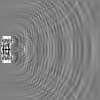
\includegraphics[width=8cm]{refraction.jpg}
  \end{figure}
  
\end{document}